
\documentclass[tikz, border=1mm]{standalone}

\usepackage{amsmath}

\usepackage{tikz}

\usetikzlibrary{calc,angles,quotes,shapes.geometric}

\usepackage{tkz-euclide}

\begin{document}

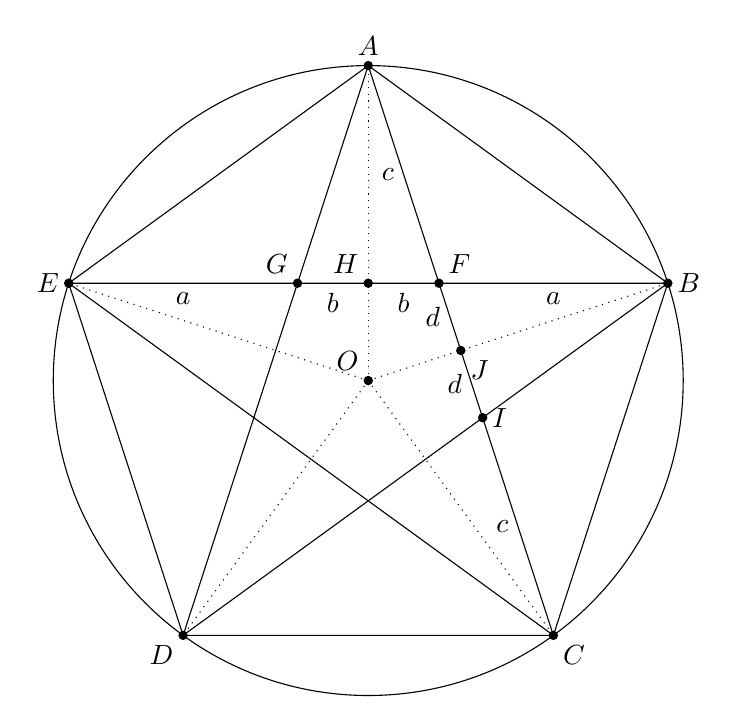
\begin{tikzpicture}[scale=2.0]

	% ---- parameters

	\def\numsides{5}
	\def\radius{2}
	\def\rotation{90}

	% ---- coordinates

	\coordinate (O) at (0,0);
	\draw (O) circle (\radius);

	\foreach \i in {1,...,\numsides} {
		\coordinate (P\i) at ({360/\numsides*(\i-1)+\rotation}:\radius);
	}

	% ---- intersections

	\tkzInterLL(P2,P5)(P1,P4)\tkzGetPoint{F}
	\tkzInterLL(P2,P5)(P1,P3)\tkzGetPoint{G}
	\tkzInterLL(O,P1)(P2,P5)\tkzGetPoint{H}

	\tkzInterLL(P3,P5)(P1,P4)\tkzGetPoint{I}
	\tkzInterLL(O,P5)(P1,P4)\tkzGetPoint{J}

	% ---- pentagon

	\draw (P1) \foreach \i in {2,...,\numsides} { -- (P\i) } -- cycle;

	% ---- radiuses

	\foreach \i in {1,...,\numsides} { \draw[dotted] (O) -- (P\i); }

	% ---- pentagram

	\draw (P1) -- (P3) -- (P5) -- (P2) -- (P4) -- cycle;

	% ---- thick vertices

	\fill (O) circle (0.3mm);
	\fill (F) circle (0.3mm);
	\fill (G) circle (0.3mm);
	\fill (H) circle (0.3mm);
	\fill (I) circle (0.3mm);
	\fill (J) circle (0.3mm);
	\foreach \i in {1,...,\numsides} { \fill (P\i) circle (0.3mm); }

	% ---- vertices labels

	\node[above left] at (O) {$O$};
	\node[above right] at (F) {$F$};
	\node[above left] at (G) {$G$};
	\node[above left] at (H) {$H$};
	\node[right] at (I) {$I$};
	\node[below right] at (J) {$J$};

	\node[above] at (P1) {$A$};
	\node[right] at (P5) {$B$};
	\node[below right] at (P4) {$C$};
	\node[below left] at (P3) {$D$};
	\node[left] at (P2) {$E$};

	\node[below] at ($(P2)!0.5!(G)$) {$a$};
	\node[below] at ($(G)!0.5!(H)$) {$b$};
	\node[below] at ($(H)!0.5!(F)$) {$b$};
	\node[below] at ($(F)!0.5!(P5)$) {$a$};

	\node[left] at ($(P1)!0.5!(F)$) {$c$};
	\node[left] at ($(F)!0.5!(J)$) {$d$};
	\node[left] at ($(J)!0.5!(I)$) {$d$};
	\node[left] at ($(I)!0.5!(P4)$) {$c$};

\end{tikzpicture}

\end{document}
